%!TEX root = practica.tex
%===============================================================================
\chapter{Set up}\label{ch:Setup}
\addcontentsline{toc}{chapter}{Set up}
%----------------------------------------------------------------------


\section{Install a native programming environment}
\addcontentsline{toc}{section}{Install a native programming environment}

The aim of this assignment is to
install a native programming environment
for the Ada language on the student's PC.
This environment will later be extended with cross-compilation tools
for the STM32 board to be used in the laboratory.

The programming environment is the GNAT Community version,
an open-source software development environment freely available from AdaCore,
a company specialized in providing tools
and solutions for developing high-integrity software.

% -- GNAT -----------------------------------------------------------------------

\subsection{Download and install GNAT}
The GNAT Community compilation system can be downloaded from \url{https://www.adacore.com/download/more}.
Installation packages for Windows, MacOS and GNU Linux
are available at the download page.
The file \texttt{README.txt} provides installation instructions,
which are summarized in the following subsections:

\subsubsection*{Windows}
\begin{enumerate}
\item Download the file \href{https://community.download.adacore.com/v1/797dbae8bdb8a3f661dad78dd73d8e40218a68d8?filename=gnat-2021-20210519-x86\_64-windows64-bin.exe\&rand=1472}{\texttt{gnat-2021-20210519-x86\_64-windows64-bin.exe}}

\item Run the file and follow the instructions.
\end{enumerate}

\textbf{\textcolor{mRedBrown}{Important}}:
GNATStudio installs additional configuration files in the \texttt{.gnatstudio} folder,
which is located under your Home directory (e.g.: \texttt{C:\textbackslash{}\textbackslash{}user\_name\textbackslash{}.gnatstudio}).
Notice that the application will not start if your user account contains special character such as spaces or accent marks.
Then, to solve this you must remove all special characters from your user account.
This 
\href{https://superuser.com/questions/890812/how-to-rename-the-user-folder-in-windows-10/1346983#1346983}
{link}
provides detailed instructions to solve this issue.

\subsubsection*{MacOS}
\begin{enumerate}
\item Download the file \texttt{gnat-2020-20200818-x86\_64-darwin-bin.dmg}
\item Open the dmg disk and execute the application inside it.
In order to circumvent the system protection,
control-click on the file and then click on ``opens" in the emergent window.
\end{enumerate}

Notice that you need to have installed the Xcode application to install GNAT.
If you still see the following error:

\begin{BVerbatim}
	ld: library not found for -lSystem
\end{BVerbatim}
\\

then you might have to execute the following:

\begin{BVerbatim}
	xcode-select -s /Applications/Xcode.app/Contents/Developer
\end{BVerbatim}

\subsubsection*{GNU Linux}
\begin{enumerate}
\item Download the file \texttt{gnat-2021-20210519-x86\_64-linux-bin}
\item You will need provide execution permissions to the binary in order to run it.
Run the following command in your terminal:

\begin{BVerbatim}
     chmod +x path_to_the_package.bin
\end{BVerbatim}

and execute the package. The \texttt{README.txt} file
contains additional installation and execution instructions.
\end{enumerate}

\subsection{Test the installation with a simple program}

The GNAT compilation system includes the
GPS (GNAT Programming Studio) integrated development environment,
which allows users to edit, compile, and run Ada and C programs. Figure\ref{fig:gps} shows the main GPS window,
which is composed of the following areas:

\begin{figure}[hbtp!]
    \centering{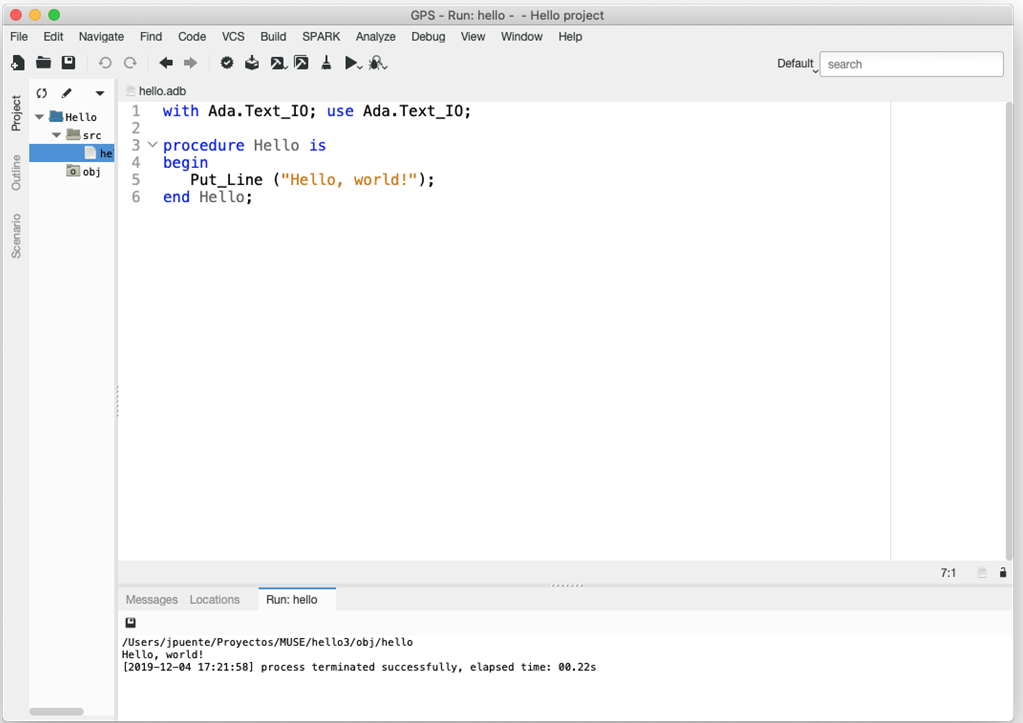
\includegraphics[width=\textwidth,keepaspectratio]{gps.png}}
    \caption{GNAT Programming Studio (GPS).}
    \label{fig:gps}
\end{figure}

\begin{itemize}
\item	a menu bar at the top
\item	a tool bar under the menu bar
\item	on the left, a notebook allowing you to switch between Project, Outline and Scenario views
\item	the working area in the center
\item	the messages window at the bottom
\end{itemize}

GPS organizes source code in projects.
A project is a set of source files which are compiled together
in order to produce a single binary executable.
Before starting you will need to create a folder to store your software projects.
The recommendation is to create a folder named
\textcolor{mPurple}{\texttt{SEU-OBDH-Lab}}
in the location of your choice.

The next activity consists on writing and running a simple Ada program with GPS:
\begin{enumerate}
\item 	Create a new project by clicking on File $\rightarrow$ New Project ...
        in the top menu. Choose the Simple Ada Project template.

\item	Choose a folder to deploy the project, e.g. \textcolor{mPurple}{\texttt{SEU-OBDH-Lab/lab-1}}.
        Set the project's name to \texttt{Hello} and the main name also to \texttt{Hello}.
        
\item	Double click on the \texttt{hello.adb} file in the project view to open the file in the working area.

\item	Edit the file in the working area so that it has the same content as in figure~\ref{fig:gps}.

\item	Build and run the executable by clicking on the $\rhd$ symbol in the tool bar.
You should see a number of compilation-related messages and,
if everything is right, you will see the text \texttt{Hello, world!}
in the Run tab of the bottom window.
\end{enumerate}
%\begin{figure}[h]
%            \centering{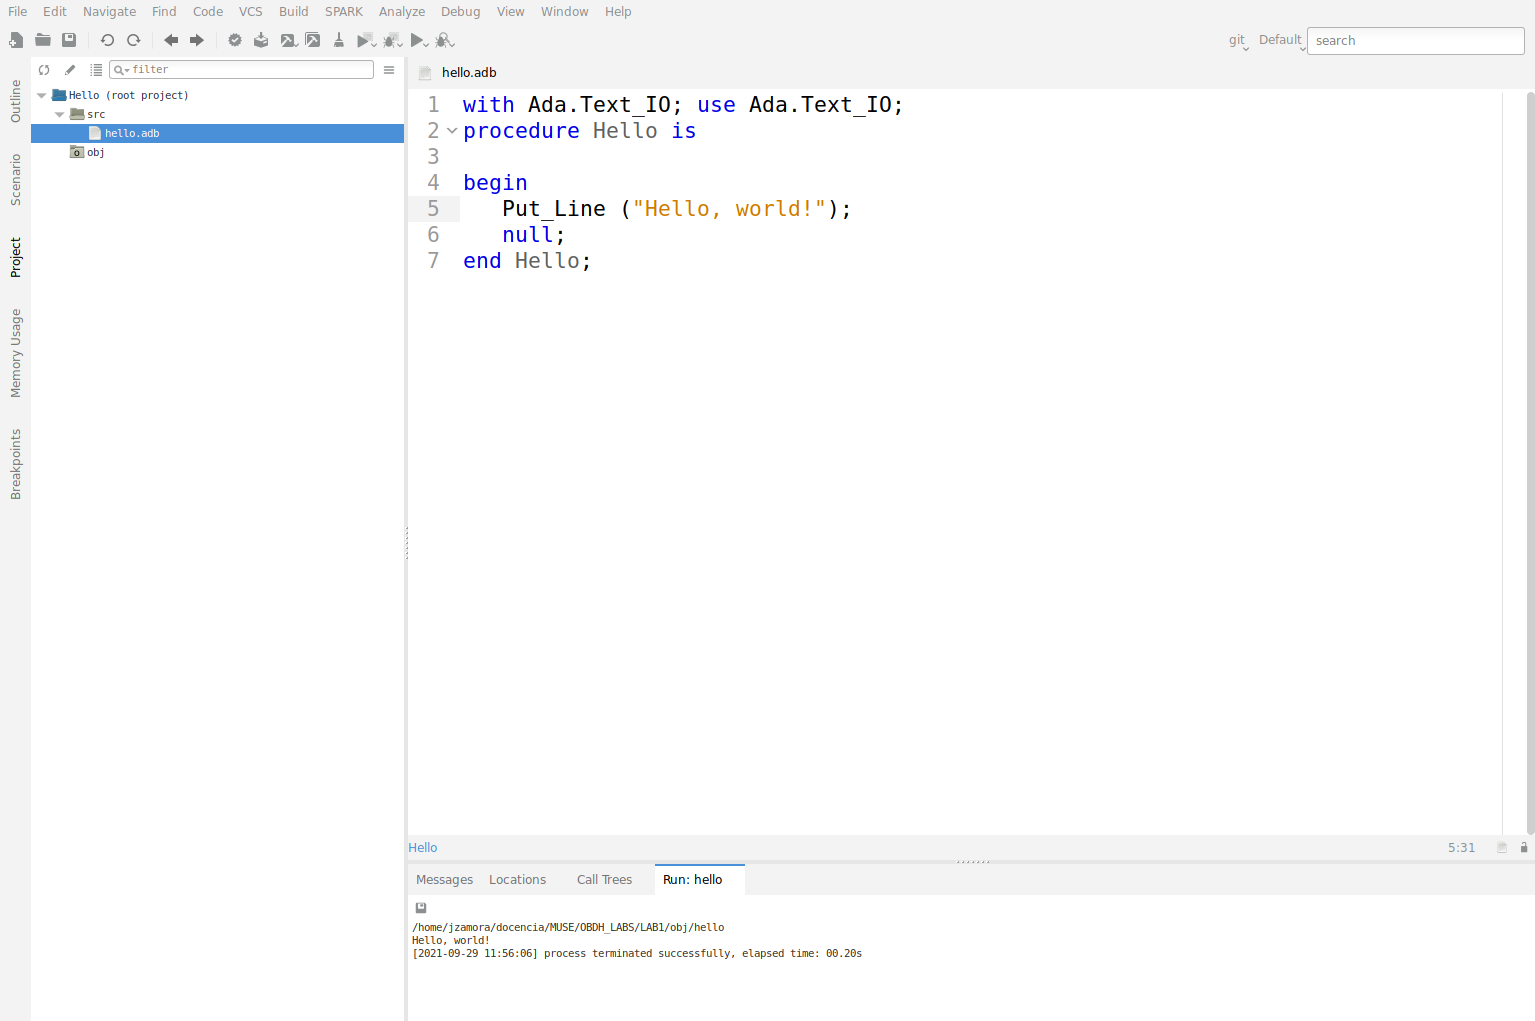
\includegraphics[width=\textwidth,keepaspectratio]{gpshello.png}}
%            \caption{Hello world demo program.}
%            \label{fig:gpshello}
%\end{figure}

\section{Install the cross-compilation tools}
\addcontentsline{toc}{section}{Install the cross-compilation tools}

The aim is to get acquainted with the embedded computer board
and to install and test the cross-compilation tools for GNAT
that will be used to develop executable code for it.

\subsection{Cross-compilation tools}

The computer board will programmed in Ada,
a systems programming language suitable for high-integrity applications.
The GNAT cross-platform development system
will be used to compile the software in the student's PC (aka. the host platform)
so that it can be uploaded in the SMT32 board (the target platform).

\begin{figure}[hbtp!]
    \centering{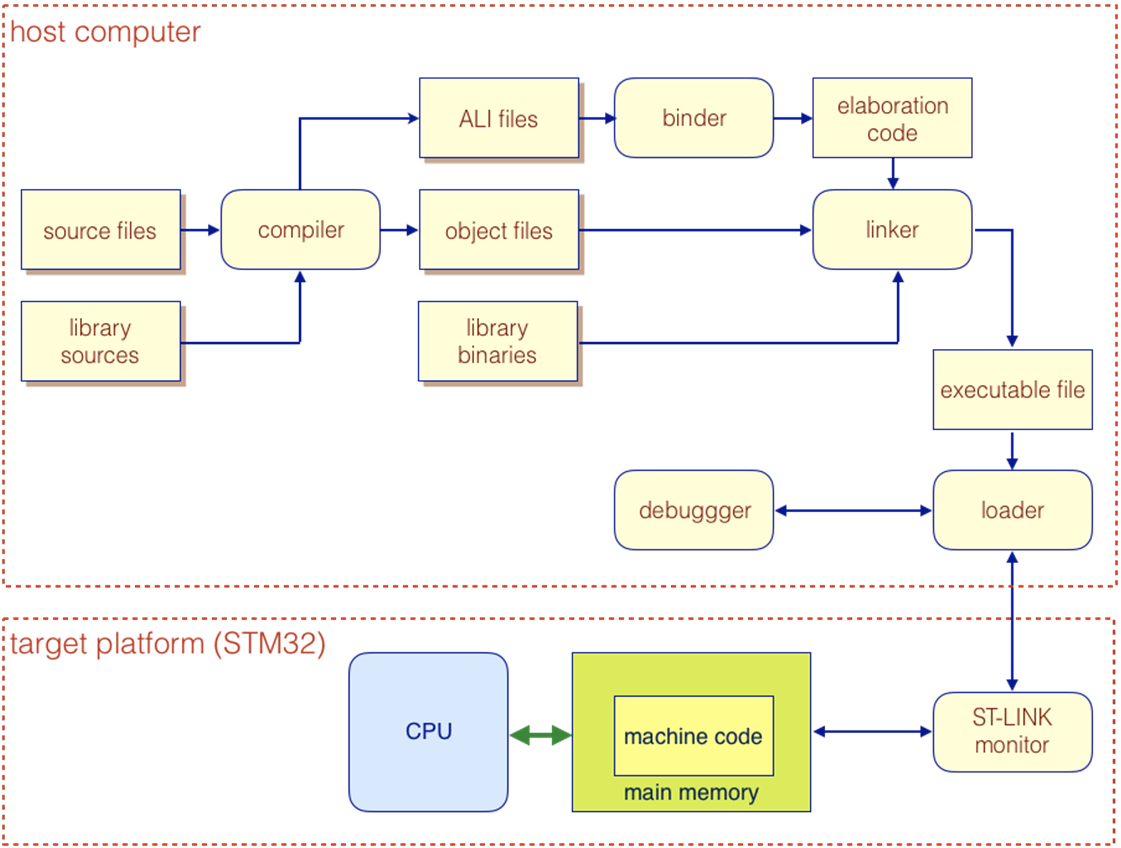
\includegraphics[width=\textwidth,keepaspectratio]{cross.png}}
    \caption{Cross-compilation and debugging system}
    \label{fig:cross}
\end{figure}

In order to compile a program, the compilation chain is run on the host computer to produce an executable file suitable for the target computer.
The executable is then loaded into the target memory,
from where it can be executed.
A monitor program is preinstalled on the target board
that supports loading and debugging from the host platform.

\subsection{Download and install GNAT ARM ELF}

GNAT ARM ELF is the cross-compilation chain to be used with the STM32F4 board. It can be downloaded from the
\href{https://www.adacore.com/download/more}{same page as the native GNAT system},
and there are installation packages for Windows, MacOS and GNU Linux available.
The file \texttt{README.txt} provides installation instructions,
which are summarized as follows.

\subsubsection*{Windows}
\begin{enumerate}
\item Select ARM ELF (hosted on windows64) and download the file
gnat-2021-20210519-arm-elf-windows64-bin.exe
\item Run the file and follow the instructions.
\item You will also need to install the USB driver for the ST-LINK probe. To do so, go to \url{http://www.st.com/content/st\_com/en/products/embedded-software/development-tool-software/stsw-link009.html}, and click on Get Software. Click on Get Software under the Download column of the table that shows up to obtain the driver. You will need to accept ST Micro’s license agreement and enter your contact details. 
Once downloaded unzip the USB device driver and run the installer, accepting all the defaults.
\end{enumerate}
\subsubsection*{MacOS}
\begin{enumerate}
\item Download the file gnat-community-2019-20190517-arm-elf-darwin-bin.dmg
\item Open the dmg disk and execute the application inside it. In order to circumvent the system protection, control-click on the file and then click on ``open" in the emergent window.
\item You will also need the st-util,  st-flash, and st-info tools. You can download the binaries from 
\url{https://github.com/texane/stlink/releases/download/1.3.0/stlink-1.3.0-macosx-amd64.zip}. Unzip and copy the files in the bin directory to a directory in your PATH. You may need to circumvent MacOS protection by executing the command:

	\$ xattr -d com.apple.quarantine path-to-executable-file
\end{enumerate}
\subsubsection*{GNU Linux}
\begin{enumerate}
\item Download the file gnat-2021-20210519-arm-elf-linux64-bin
\item You will need to make the package executable before running it. In a command prompt, execute the following command:

     chmod +x path\_to\_the\_package.bin

and then execute the package.
\item You will also need to install the stlink tools. In Ubuntu and Debian stlink must be installed from sources. Follow the instructions on \url{http://docs.adacore.com/live/wave/gnat\_ugx/html/gnat\_ugx/gnat\_ugx/arm-elf\_topics\_and\_tutorial.html\#linux}.
\end{enumerate}

The README.txt file contains additional installation and execution instructions.

\subsection{Test your installation with an embedded program}

The next thing is to compile a run a simple embedded program. This program is only intended to test that the compilation chain and the ST-LINK tools have been properly installed.

Open GPS and do the following:
\begin{enumerate}
\item Create a new project by clicking on File $\rightarrow$ New Project ... in the top menu. Choose the STM324F compatible $\rightarrow$ LED demo project template.
\item	Choose a folder to deploy the project, e.g. \texttt{SEU-OBDH-Lab/ass-2}. Set the project name to led\_demo and the main name to main. A window with a project including a number of source files will open.
\item	Right-click on the project icon on the left side area, and choose Project $\rightarrow$ Properties (figure 6). On the emerging window, select Embedded and change the Connection tool selector to st-util. Save the settings.
\item	Connect the STM32F4 board to the computer by means of a USB A / mini USB cable.
\item	Build the executable and load it into the board by clicking on the
\hbox{
\includegraphics[width=1.5em]{buildandload.png}} symbol in the tool bar (or select Build $\rightarrow$ Bareboard $\rightarrow$ Flash to board on the top menu). You should see a number of compilation-related messages ending with ``Flashing complete. You may need to reset or cycle power".
\item	If everything is all right, you will see the LEDS on the board blinking in a circular pattern.
\item Download and install the Ada Drivers Library
The Ada Drivers Library is a set of Ada packages that make it easier to write software for embedded devices, including the STM32F4 microcontroller family and some demonstration boards. The source code can be found at \url{https://github.com/AdaCore/Ada\_Drivers\_Library}. To install the library, click on the green Clone or download button on the upper right side and then on Download Zip in the emerging window. You will get a zip archive in your downloads folder. Unzip the archive and move the resulting folder to your SEU-OBDH-Lab folder. Rename the folder to Ada\_Drivers\_Library, removing any trailing text.
\item Compile and run a test program with the Ada Drivers Library
\end{enumerate}
Open GPS and do the following:
\begin{enumerate}
\item Select Open project on the welcome window. Navigate to

\begin{BVerbatim}
	.../SEU-OBDH-Lab/-Ada_Drivers_Library/examples/STMF4_DISCO
\end{BVerbatim}

and open the project file named \texttt{blinky\_f4disco.gpr}

\item	Build the executable and load it into the board by clicking on the \hbox{
\includegraphics[width=1.5em]{buildandload.png}} symbol in the tool bar (or select Build $\rightarrow$ Bareboard $\rightarrow$ Flash to board on the top menu). When the loading is complete, you will see the board LEDS blinking all at the same time.
\end{enumerate}

\section{Install MATLAB\texttrademark and Simulink\texttrademark}
\addcontentsline{toc}{section}{Install MATLAB\texttrademark and Simulink\texttrademark}

MATLAB and Simulink will be used to generate C code from a Simulink model and 
to validate the system by the Processor In the Loop (PIL) technique. The UPM has a campus license available for students.
Please read this \href{https://www.upm.es/sfs/Rectorado/Vicerrectorado\%20de\%20Tecnologias\%20de\%20la\%20Informacion\%20y\%20Servicios\%20en\%20Red/Servicio\%20de\%20Planificacion\%20Informatica\%20y\%20Comunicaciones/SW/MATLAB\_UPM\_Estudiantes.pdf}{document} to access and install MATLAB with the UPM's license.

\textbf{\textcolor{mRedBrown}{Important:}} Please, consider the following notes:
\begin{itemize}
\item The complete installation of MATLAB, including add-ons, requires approximately 10 GB.

\item Choose the Individual License, not the Concurrent.

\item During the installation procedure, on the 3rd tab of \textbf{products}, install the following \textbf{add-ons}:
\begin{itemize}
	 \item MATLAB
	 \item Simulink
	 \item MATLAB Coder
	 \item Simulink Coder
	 \item Aerospace Toolbox
\end{itemize}

\item After the full installation, the \textbf{Embedded Coder} add-on must be installed.
\end{itemize}
